\section{Data and study area}
\subsection{LiDAR and orthophoto data}
Raw LiDAR point cloud data were retrieved from ``Publieke Dienstverlening op de Kaart'' (PDOK), an open geo-information service of the Dutch government.\footnote{https://www.pdok.nl/nl/ahn3-downloads} The data are part of the ``Actueel Hoogtebestand Nederland 3'' (AHN3) dataset, which is collected between 2014 and 2019. The point density is on average over 10 points/m$^2$  and includes multiple discrete return values as well as intensity data. The dataset is collected in the first quarter of each year when deciduous vegetation is leafless \citep{AHN2016inwinjaren}. Nevertheless, the return signal is sufficiently strong to retrieve a useful scan of the vegetation cover. Freely available very high resolution (VHR) true color orthophotos from PDOK with a resolution of 25cm were consulted for validation purposes.\footnote{https://www.pdok.nl/nl/service/wms-luchtfoto-beeldmateriaal-pdok-25-cm-rgb}

All data were analyzed using free and open source software.\footnote{https://github.com/clucas111/delineating-linear-elements} The scripting was performed in Python (3.6.4) using the NumPy (1.13.3) \citep{walt2011numpy}, SciPy (1.0.0) \citep{jones2001scipy}, pandas (0.20.3) \citep{mckinney2010data}, and scikit-learn (0.19.1) \citep{pedregosa2011scikit} libraries. For the preprocessing of data, the software LASTools (version 160429) and CloudCompare (v2.10beta) were used. CloudCompare was also used for visualizing and down-sampling the point cloud.

\begin{figure}
	\centering
	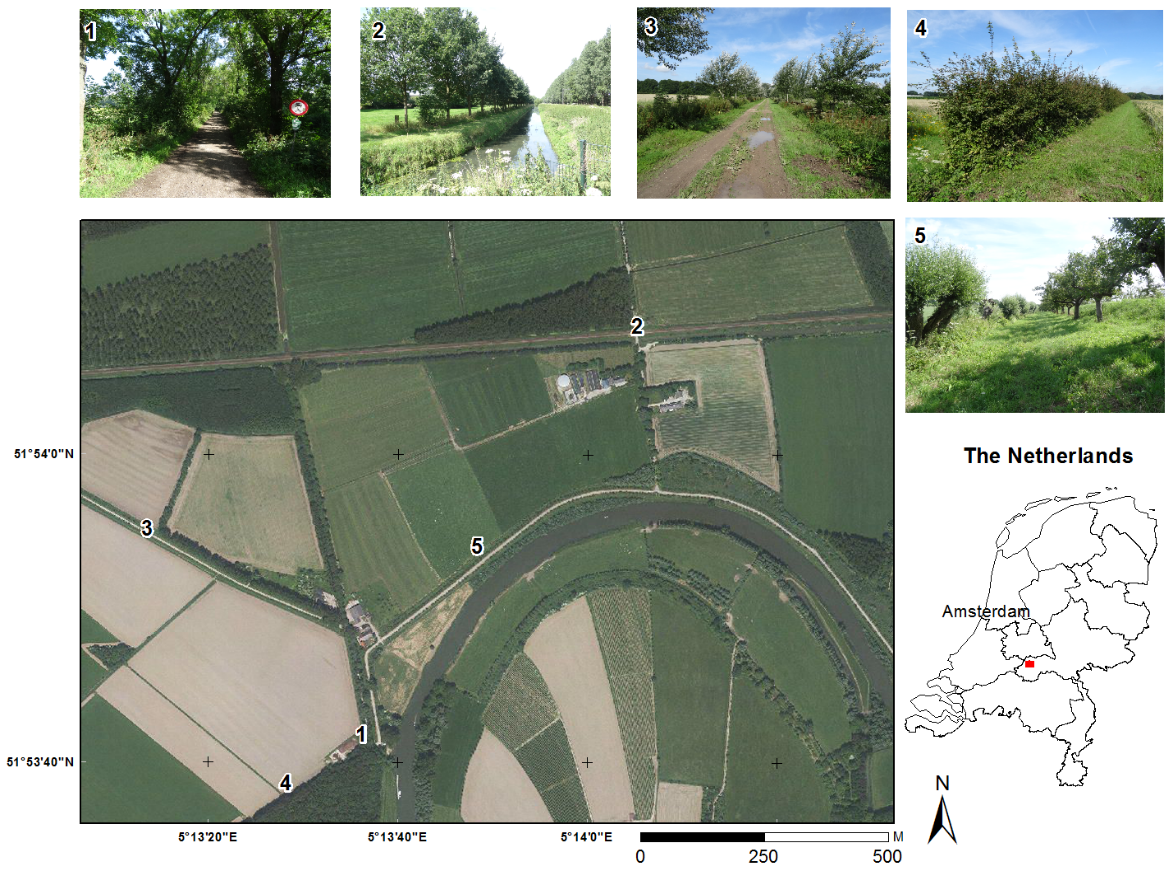
\includegraphics[scale=0.8]{./img/studyarea}
	\caption{Location of the study area in the central part of The Netherlands. The true color aerial photo (PDOK) shows several linear objects in the rural landscape related to agricultural fields, grasslands, bare soil and infrastructure such as (un)paved roads and farmhouses. The numbered photo insets show a selection of the variety of linear vegetation elements, such as green lanes (photo 1), planted high tree lines along ditches, low and high shrubs/copse (photo 3), hedges (photo 4) and isolated traditional fruit trees.}
	\label{fig:studyarea}
\end{figure}

\subsection{Study area}
The case study area is located in a rural landscape in the center of the Netherlands south of Amsterdam (figure \ref{fig:studyarea}). The area is about 1.6 km from east to west and 1.2 km from north to south, spanning an area of almost 2 million square meters. The point density of the point cloud in the area is 22.49 points/m$^2$. The area contains numerous woody linear objects of varying geometry, ranging from completely straight to curved, isolated or connected to other linear or non-linear objects. Examples of vegetation and non-vegetation elements are planted forest patches, hedges, green lanes, isolated farms, ditches, a river, dykes and a road network (figure \ref{fig:studyarea}). This heterogeneity within a small area ensured that both the classification of vegetation and delineation of linear objects can be efficiently trained and tested.